
%(BEGIN_QUESTION)
% Copyright 2015, Tony R. Kuphaldt, released under the Creative Commons Attribution License (v 1.0)
% This means you may do almost anything with this work of mine, so long as you give me proper credit

During the 1980's the Rosemount corporation developed a means for 4-20 mA analog signaling circuits to carry digital signals as well, so that 4-20 mA process transmitters could be equipped with microprocessors and communicate data in both analog and digital form.  Rosemount's so-called {\it HART} standard (``Highway-Addressable Remote Transducer'') used audio-frequency AC signals to represent binary ``1'' and ``0'' states, superimposing these AC signals on the same two wires as the DC 4-20 mA analog signal.  Process transmitters so equipped were dubbed {\it smart transmitters} because their internal microprocessors gave them extra capabilities such as self-diagnostics, easy-to-change ranging, and advanced linearization for greater accuracy.  HART eventually became an ``open'' standard with many manufacturers producing compliant field devices.

\vskip 10pt

The following schematic diagram shows a simplified HART transmitter connected to a DC loop power supply as well as a HART ``communicator'' device allowing a human technician to communicate with the transmitter.  The transistor states shown in this diagram reflect the master (``communicator'') device sending data while the slave (smart transmitter) device listens:

$$\includegraphics[width=15.5cm]{i03876x01.eps}$$

Since this is a multi-source circuit, with {\it four} sources (one AC current source and one DC current source inside the smart transmitter, one AC voltage source in the HART communicator, and one DC voltage source providing loop power), we may apply the {\it Superposition Theorem} to determine the combined effect of these sources together in one circuit.

\vskip 10pt

Use the Superposition Theorem to determine the voltage seen by the indicator, assuming the transmitter happens to be outputting a 50\% (12 mA) analog signal, and the HART communicator happens to be outputting a 400 mV AC signal at 2200 Hz at the moment of our analysis.

\underbar{file i03876}
%(END_QUESTION)





%(BEGIN_ANSWER)

Recall that the Superposition Theorem works by considering one source at a time, with all other sources ``disabled'' and replaced by their respective internal impedances.  With four sources, this means we must analyze the circuit four times over (once for each active source), and then superimpose the results of all four analyses.

%(END_ANSWER)





%(BEGIN_NOTES)

\noindent
{\bf Analysis \#1:} (DC loop power source only)

$$\includegraphics[width=15.5cm]{i03876x02.eps}$$

Here, we see what the loop power supply does on its own, with all current sources opened (infinite internal impedance) and all other voltage sources shorted (zero internal impedance).  The result is an open circuit, with nothing dropped across the 250 ohm resistor.

\filbreak

\noindent
{\bf Analysis \#2:} (HART communicator source only)

$$\includegraphics[width=15.5cm]{i03876x03.eps}$$

Here, we see what the HART communicator's AC voltage source does on its own, with all current sources opened (infinite internal impedance) and all other voltage sources shorted (zero internal impedance).  The result is the communicator's AC voltage dropped entirely across the resistor (and also seen across the terminals of the smart transmitter where the microprocessor will be able to read it).  We are assuming that the coupling capacitor's impedance is negligible.

\filbreak

\noindent
{\bf Analysis \#3:} (transmitter analog source only)

$$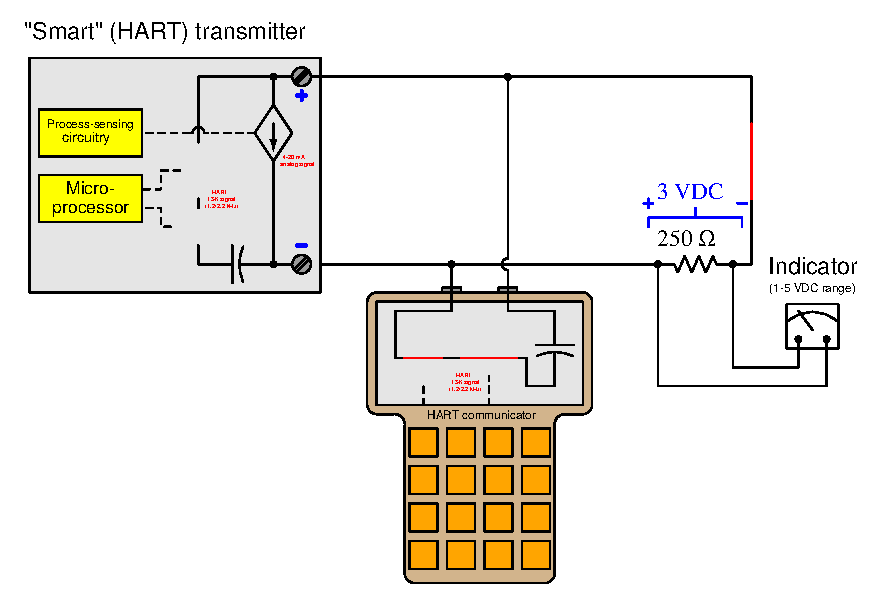
\includegraphics[width=15.5cm]{i03876x04.eps}$$

Here, we see what the smart transmitter's DC current source does on its own, with all other current sources opened (infinite internal impedance) and all voltage sources shorted (zero internal impedance).  The result is a 3 volt drop across the resistor based on Ohm's Law ($V = IR$ = 12 mA $\times$ 250 $\Omega$ = 3 volts). 

\filbreak

\noindent
{\bf Analysis \#4:} (transmitter HART source only)

$$\includegraphics[width=15.5cm]{i03876x05.eps}$$

Here, we see what the smart transmitter's AC current source does on its own, with all other current sources opened (infinite internal impedance) and all voltage sources shorted (zero internal impedance).  The result is nothing, since the MOSFET in series with this source is turned off.

\vskip 10pt

Superimposing all these results together, we see that the indicator experiences a composite DC+AC signal of 3 volts DC and 400 mV AC at 2200 Hz.

%INDEX% Fieldbus, HART: analysis of 4-20 mA / HART transmitter circuit using Superposition Theorem

%(END_NOTES)


